\section{Statistical methods}\label{sec:stats_methods}
A list of states as ranked by internet connectivity may be of interest to a casual reader of our results. Unfortunately, due to complications in the data and the nature of aggregation by arbitrary political boundaries, this process is not as simple as conducting a sort.

\subsection{Kruskal-Wallis test}

Regardless of the method of data collection used, if aggregating by state the data will inevitably become a list of data points for each possible state. However, states are \textit{massive} regions with varying populations, infrastructure, etc. and there is as of yet no reason to believe that there is a causal relationship between states and the internet connectivity found there. This means that within any state grouping there may be a large amount of variation and a potentially complex distribution. For this reason a proper statistical test is needed.

The requirements are simple: a non-parametric (i.e. does not assume a normal distribution) test that determines if a ranking of two or more categorical variables is impossible, on variables with unequal sample sizes. The chosen test that meets these requirements is the Kruskal-Wallis \textit{H} test, also known as a one-way \anova on ranks. When used on a data set, the result is a \textit{H} value that, assuming a chi-squared distribution, can be used to calculate a $p$ value \cite{kruskal-wallis}. In this case $p$ should be interpreted as the probability that all the given samples come from the same distribution, i.e. that we cannot tell a difference between them. For a more concrete example, if we run the Kruskal-Wallis test on samples for the states of California and Tennessee and obtain $p=0.75$, there's a 75\% probability that the two states' values come from the same distribution. This report uses the $p<0.05$ level for its analyses, so in this case the two states would be deemed indistinguishable.

\subsection{Distinguishability Graphs}

The Kruskal-Wallis test cannot tell us if a ranking of 3+ variables is possible, only that one sample dominates the others \cite{kruskal-wallis}. This means that in a sample of 51 categorical variables\footnote{50 states + the District of Columbia.} the $p$ value may be very low, but not all states can be directly compared. An important property of an ordered list is that any two values should be comparable to all those before and after it in a meaningful way. A traditional sorting algorithm running on means or medians cannot be applied, as there is no way to control whether it will try to compare states that the Kruskal-Wallis test says cannot be distinguished at the $p<0.05$ level.

To visualize this we developed the concept of a distinguishability graph. Briefly, states can be interpreted as vertices on a graph, and pairwise comparisons that are valid or invalid based on the Kruskal-Wallis test can be visualized as edges. With some processing from the SciPy toolkit, Pandas, and visualization + arrangement done by NetworkX or D3 \cite{scipy, pandas, networkx, Bostock2011a}, we can generate graphs showing these relationships and relevant attributes.

\begin{figure}[h]
    \centering
    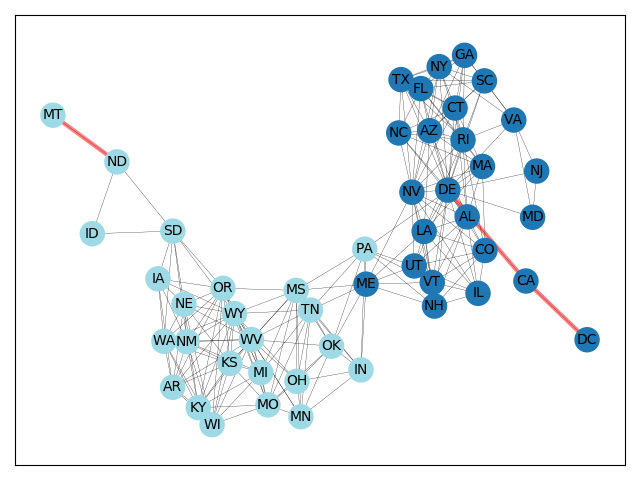
\includegraphics[width=0.66\textwidth]{caida/caida_network_invalid_comps.png}
    \repeatcaption{fig:caida_network_invalid_comps}{Indistinguishability graph (at $p\geq0.05$) for pairwise state comparisons}
\end{figure}

\Cref{fig:caida_network_invalid_comps} shows an example of such a graph, for pairwise state comparisons. Each edge between states represents a comparison that \textit{cannot} be made (making this an \textbf{in}distinguish\-ability graph), red-highlighted edges are bridges, and node colors correspond to the community that node belongs to. On this particular graph there are no disjoint subgraphs, so ranking by clusters of states is not possible. In graphs where their are disjoint subgraphs, however, ranking by clustered states would be possible.

\begin{figure}[h]
    \centering
    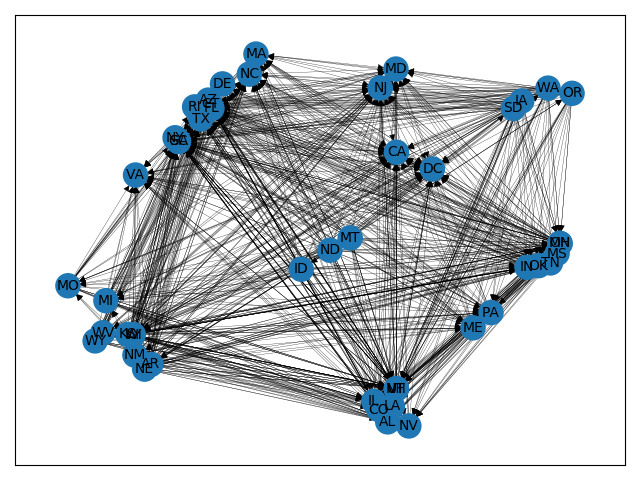
\includegraphics[width=0.66\textwidth]{images/caida/caida_network_valid_comps.png}
    \repeatcaption{fig:caida_network_valid_comps}{Distinguishability graph (at $p<0.05$) for pairwise state comparisons}
\end{figure}

\Cref{fig:caida_network_valid_comps} shows an example of a distinguishability graph at the $p<0.05$ level; since edges here represent comparisons between states that \textit{are} distinguishable, this graph is drawn as a directed graph. The direction of the edge follows the order of which state has better connectivity (the ancestor of a node has better connectivity). This opens up new possibilities for the ranking of states \textit{without} relying on traditional sorting algorithms.

\subsection{Topologically-sorted state rankings}\label{sec:methods_stats_topological_rankings}

% \todo{Move to CAIDA section}
A graph of states that are distinguishable is most naturally represented as a directed graph. When conducting comparisons it's possible to calculate a ratio between the states based on the fraction of connectivity quality that the worse state has to the second (a value ranging from 0-1). These ratios can be used as weights along edges between states, allowing a topological sort of the graph to be conducted. Edges with weights that are higher are explored first (since they correspond to states that are closer to being equal). The result may not be entirely intuitive at first and undoubtedly has some oddities from the unusual sorting method, but may be useful in addition to a simple mean/median-based sort.

One drawback of the topological sort method is that it implicitly compares states that according to the Kruskal-Wallis test cannot actually be compared. For instance, if you have $CA\rightarrow MA$ and $CA\rightarrow TX$, but the comparison between $MA$ and $TX$ isn't supported by the data, the topological sort method must choose between them somehow. That choosing process is an implicit comparison, making the topological sort method a rough guess at state rankings at best.

\subsection{Z-Score Filtering} \label{sec:z-score-filtering}

To filter out statistical outliers from our data sets we choose use a technique known as z-score filtering. Z-score filtering works by calculating the standard deviation of a data set and then removing values that are greater then a set number of standard deviations away from the mean. The z-score is number of standard deviations away as data point needs to be for it to be considered an outlier. For this report, we choose to use a z-score value of 2, and therefor 95\% of the data will be preserved.
